\section {Implementation and Technical Notes}

The code was run on a \textit{GTX 1080 Ti} and not the cluster of \textit{K'40s}. This could be a reason for variance in the optimal configuration found for the GPUs. However, the code does not make any hardware assumptions and can therefore be run on any suitable cluster. \\

CUDA version 9.0 was used to compile the code, with \lstinline{nvcc} as the device compiler and \lstinline{gcc} as the host compiler.

\section {Question 1 and 2}

Matrix Multiplication via thread-wise access to global memory was used. \\

We implement two matrix multiplication kernels: one for column major access ( fastest varying y) and one for row major access (fastest varying x). We utilise \textit{Cuda Events } to time the two runs. The results may be replicated by running,

\begin{lstlisting}[numbers = none]
./ee16b068_1.cu
\end{lstlisting}

\subsection{Run Timing and Interpretation}

\begin{lstlisting}[numbers = none]
Time spent in col maj 28395.593750

Time spent in row maj 46189.101562
\end{lstlisting}

This can be attributed to the fact that DRAM bursts are more efficiently accessed with simultaneous access to the same row. For parallel access this means each thread should ideally access different rows with time, but the same row spatially. Hence, column major outperforms row major. \\

For questions 2,3 , we shall consider column major timing only. \\

\subsection {Code Blocks (pertinent only)}
\begin{lstlisting}
__global__ void MatrixMulKernel_col_maj(double* M, double* N, double* P, int Width) { 
    // Calculate the row index of the P element and M
    int Row = blockIdx.y*blockDim.y+threadIdx.y;
    // Calculate the column index of P and N
    int Col = blockIdx.x*blockDim.x+threadIdx.x; 
    
    if ((Row < Width) && (Col < Width)) {
            float Pvalue = 0;
        for (int k = 0; k < Width; ++k) {
            Pvalue += M[Row*Width+k]*N[k*Width+Col];
        }
            P[Row*Width+Col] = Pvalue;
        }
    }

__global__ void MatrixMulKernel_row_maj(double* M, double* N, double* P, int Width) { 
    // Calculate the row index of the P element and M
    int Row = blockIdx.y*blockDim.y+threadIdx.x;
    // Calculate the column index of P and N
    int Col = blockIdx.x*blockDim.x+threadIdx.y; 
    
    if ((Row < Width) && (Col < Width)) {
            float Pvalue = 0;
        for (int k = 0; k < Width; ++k) {
            Pvalue += M[Row*Width+k]*N[k*Width+Col];
        }
            P[Row*Width+Col] = Pvalue;
        }
    }

\end{lstlisting}
\bigskip

\section{Question 2}

We now use similar code to question 1, except, varying threadsPerBlock as a parameter, from 4 to 32. (We could use up to 1024 threads a block, and for two dimensional threads, this is $32^2$). Nevertheless, we include upto 128, and note any errors. \\

Corresponding plot in \textbf{Figure 1}\\

The noted performance is:

\begin{figure}[ht]
\centering
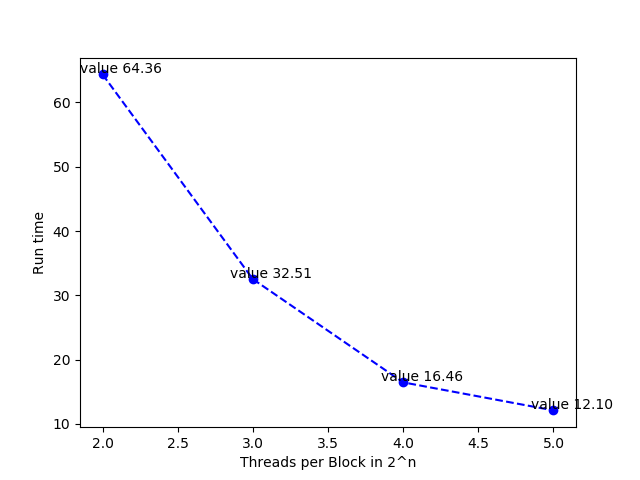
\includegraphics[angle=0,width=0.7\textwidth]{assignment-2/report/q2.png}
\caption{Naive Matrix Multiplication versus Threads per Block for \textbf{GTX 1080 Ti}}
\end{figure}


\section {Question 3 }

We utilise the shared memory, however, not via tiling, but rather just using dependencies of each block.  Assuming that a block is of size $Tile Width * Tile Width$, the numbers access directly (no iterartions) are $2 * Tile Width * Matrix Width$. Note that, here for the sake of simplicity we are working with square matrices. We find the time taken for the same multiplication as in \textbf{Question 1} with this new strategy. \\

In the first part of this questionn, we use a $16 * 16$ matrix, and obtain the following:

\begin{lstlisting}[numbers = none]
Time spent in col maj 0.019232
\end{lstlisting}

In the second case, we use the original size of $8192$. Considering the smaller size of shared memory (as opposed to global memory, we expect this to fail, returning a null matrix output). \\

\textit{cudaPeekErrors} reveals the lack of sufficient shared memory in the second case. \\

\begin{lstlisting}[numbers = none]
 cudaError_t err1 = cudaPeekAtLastError();//To capture last error in function call
\end{lstlisting}

\subsection{Code Changes}

We use the concept of templates and external shared registers to dynamically declare arrays. Reference : CUDA Documentation. \\

\begin{lstlisting}
	__global__ void MatrixMulKernel_col_maj(double* M, double* N, double* P, int Width) { 
    extern __shared__ double buffer[];

    double *ds_M = &buffer[0]; // TILE_WIDTH WIDTH
    double *ds_N = &buffer[TILE_WIDTH*Width]; // WIDTH TILE_WIDTH

    //__shared__ float ds_M[Width][Width];
    //__shared__ float ds_N[Width][Width];
    int bx = blockIdx.x;  int by = blockIdx.y;
    int tx = threadIdx.x; int ty = threadIdx.y;
    int Row = by * blockDim.y + ty;
    int Col = bx * blockDim.x + tx;
    
    
    // Loop over the M and N tiles required to compute the P element
    for (int p = 0; p < Width/TILE_WIDTH; ++p) {
    // Collaborative loading of M and N tiles into shared memory
    ds_M[ty*Width + tx + p*blockDim.x ] = M[Row*Width + p*TILE_WIDTH+tx];
    ds_N[ty*TILE_WIDTH + blockDim.y*TILE_WIDTH*p + tx] = N[(p*TILE_WIDTH+ty)*Width + Col];
    __syncthreads();
    }

    double Pvalue = 0;
    for (int i = 0; i < TILE_WIDTH; ++i){
        Pvalue += ds_M[ty*Width + i] * ds_N[i*Width + tx];
    }
    __syncthreads();
    P[Row*Width+Col] = Pvalue;
}
\end{lstlisting} \\

\section {Question 4}

Here, we implement tiling for the case of similar square matrices. \\

We compare the performance boost versus question 1.

\begin{lstlisting}[numbers = none]
Time spent in col maj 4015.230225
\end{lstlisting} 

The matrix multiplication takes just 4 seconds, a major improvement over 28 seconds previously. Note that this is due to lower latency in data access and the problem of DRAM locality being efficiently addressed by tiling.

\subsection{Code Changes} 
\begin{lstlisting}
__global__ void MatrixMulKernel_col_maj(double* M, double* N, double* Q, int Width) { 
    //extern __shared__ double buffer[];
    //double *ds_M = &buffer[0];
    //double *ds_N = &buffer[Width*Width];

    __shared__ double ds_M[TILE_WIDTH][TILE_WIDTH];
    __shared__ double ds_N[TILE_WIDTH][TILE_WIDTH];

    // Generate IDs
    double Pvalue=0;
    int bx = blockIdx.x;  int by = blockIdx.y;
    int tx = threadIdx.x; int ty = threadIdx.y;
    int Row = by * blockDim.y + ty;
    int Col = bx * blockDim.x + tx;

    
    // Loop over the M and N tiles required to compute the P element
    for (int p = 0; p < (Width)/TILE_WIDTH; ++p) {
        if ( (Row < Width) && (tx + p*TILE_WIDTH) < Width){
        // Collaborative loading of M and N tiles into shared memory
        ds_M[ty][tx] = M[Row*Width + p*TILE_WIDTH+tx];
        }
        else{
            ds_M[ty][tx]=0.0;
        }
        if ( (Col < Width) && (ty + p*TILE_WIDTH) < Width){
        ds_N[ty][tx] = N[(p*TILE_WIDTH+ty)*Width + Col];
        }
        else{
            ds_N[ty][tx]=0.0;
        }
        __syncthreads();

        for (int i = 0; i < TILE_WIDTH; ++i){
            Pvalue += ds_M[ty][i] * ds_N[i][tx];
            
        }
        __syncthreads();
        
    }
    
    if ((Row < Width) && (Col < Width)){
    Q[Row*Width+Col] = Pvalue;
    }
}
\end{lstlisting} \\


\section {Question 5}

We vary the tile size from $4*4$ to $32*32$ to  find the most optimal tile size. Considering that the \textbf{GTX 1080 Ti} can fit 1024 threadsPerBlock, we expect $32$ to be the optimal tilesize. \\

Note that tilesize being varied independently of the blocksize, ... ie, having a block size as a multiple of the tile size doesnot make a difference as it now effectively acts a bigger tile. Hence the only independent parameter here is the tilesize. \\

Again, empirically, we observe that $32 *32$ is the most optimal tile size. This makes sense, since there are greater advantages with a larger tile size, and the only upperbound being the shared memory and the number of threadsPerBlock.
 
 \subsection{Run-Times}
 
 No major code changes here, besides varying the tile sizes given these optimal \textit{Threads per Block} .\\
 
 Corresponding plot in \textbf{Figure-2}.
 
 \begin{figure}[ht]
\centering
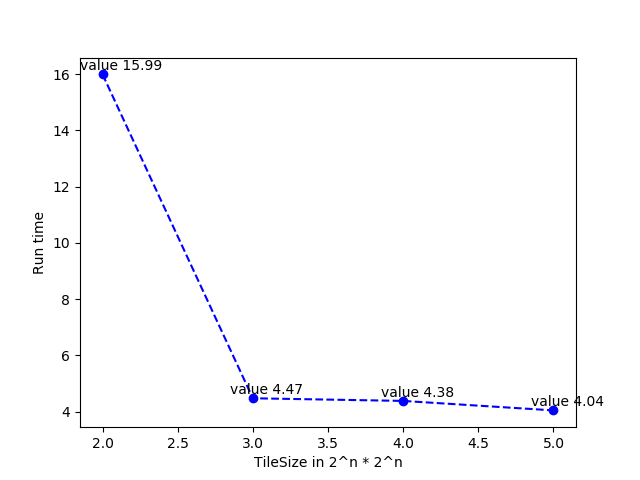
\includegraphics[angle=0,width=0.7\textwidth]{q5.png}
\caption{Average Runtime versus Tile Size for \textbf{GTX 1080 Ti}}
\end{figure}

\section{Question 6}

We generalise tiling for rectangular matrices. The changes made are primarily by matching corresponding row-column sizes as well as the correct boundaries for each tile and index.

This is more evident in the code snippet below. We try this out for a matrix multiplication of $4096 * 8192$ times $8192*16384$, and report the following runtime.

Note that this is slightly slower than 1 due to more matrix ops. Further if conditions are put in place to handle the externalities. This therefore can generalise to arbitrary multiplicand sizes.

\subsection{Code Changes} 

\begin{lstlisting}
__global__ void MatrixMulKernel_col_maj(double* M, double* N, double* Q, int M_r, int N_c, int M_c) { 
    //extern __shared__ double buffer[];
    //double *ds_M = &buffer[0];
    //double *ds_N = &buffer[Width*Width];

    __shared__ double ds_M[TILE_WIDTH][TILE_WIDTH];
    __shared__ double ds_N[TILE_WIDTH][TILE_WIDTH];

    // Generate IDs
    double Pvalue=0;
    int bx = blockIdx.x;  int by = blockIdx.y;
    int tx = threadIdx.x; int ty = threadIdx.y;
    int Row = by * blockDim.y + ty;
    int Col = bx * blockDim.x + tx;

    
    // Loop over the M and N tiles required to compute the P element
    for (int p = 0; p < (M_c)/TILE_WIDTH; ++p) {
        if ( (Row < M_r) && (tx + p*TILE_WIDTH) < M_c){
        // Collaborative loading of M and N tiles into shared memory
        ds_M[ty][tx] = M[Row*M_c + p*TILE_WIDTH+tx];
        }
        else{
            ds_M[ty][tx]=0.0;
        }
        if ( (Col < N_c) && (ty + p*TILE_WIDTH) < M_c){
        ds_N[ty][tx] = N[(p*TILE_WIDTH+ty)*N_c + Col];
        }
        else{
            ds_N[ty][tx]=0.0;
        }
        __syncthreads();

        for (int i = 0; i < TILE_WIDTH; ++i){
            Pvalue += ds_M[ty][i] * ds_N[i][tx];
            
        }
        __syncthreads();
        
    }
    
    if ((Row < M_r) && (Col < N_c)){
    Q[Row*N_c+Col] = Pvalue;
    }
}
\end{lstlisting} \\

\section{Question 7}

We use a similar structure as \textbf{Question 5} to find the most optimal configuration , here, dictated by the tile size. An array stores the time taken and empirically finds the best configuration.\\

We find the following configuration: \\

\begin{lstlisting}[numbers = none]
Optimal time is 32806.507812, threads per block is 32 x 32, tile size is 32 x 32 blocks per grid is 257 x 1025.
\end{lstlisting} 

\section{References}
\begin{itemize}
\item Classroom lectures and Slides.
\item CUDA Dev Documentation.
\end{itemize}

